\documentclass{article}

\usepackage[utf8]{inputenc}
\usepackage[T1]{fontenc}
\usepackage[a4paper, total={7in, 9.5in}]{geometry}
\usepackage{url}
\usepackage{subfigure}
\usepackage{tabularx}
\usepackage{xtab}
\usepackage{longtable}
\usepackage{ragged2e}
\usepackage{xltabular}
\usepackage{booktabs}
\usepackage{multirow}
\usepackage{grffile}
\usepackage{indentfirst}
\usepackage{caption}
\usepackage{listings}
\usepackage[ruled,linesnumbered,lined]{algorithm2e}
\usepackage[bookmarks=false]{hyperref}
\usepackage{amssymb}
\usepackage[polish]{babel}
\usepackage{csquotes}

\setlength{\parindent}{0pt}     % remove paragraph indent

\hypersetup{
    colorlinks=true,
    linkcolor=blue,
    citecolor=blue,
    urlcolor=blue
}

\title{Raport 2. - Ekspansja pożarów}
\author{Piotr Czarnik,
Szymon Ryś,
Jakub Sordyl,
Wojciech Szmelich}
\date{\today}

\usepackage{xcolor}

\definecolor{codegreen}{rgb}{0,0.6,0}
\definecolor{codegray}{rgb}{0.5,0.5,0.5}
\definecolor{codepurple}{rgb}{0.58,0,0.82}
\definecolor{backcolour}{rgb}{0.95,0.95,0.92}

\lstdefinestyle{mystyle}{
    backgroundcolor=\color{backcolour},   
    commentstyle=\color{codegreen},
    keywordstyle=\color{magenta},
    numberstyle=\tiny\color{codegray},
    stringstyle=\color{codepurple},
    basicstyle=\ttfamily\small,
    breakatwhitespace=false,         
    breaklines=true,                 
    captionpos=b,                    
    keepspaces=true,                 
    numbers=left,                    
    numbersep=5pt,                  
    showspaces=false,                
    showstringspaces=false,
    showtabs=false,                  
    tabsize=2
}
\lstset{style=mystyle}

\usepackage[
style=numeric,
sorting=nyt,
isbn=false,
doi=true,
url=true,
backref=false,
backrefstyle=none,
maxnames=10,
giveninits=true,
abbreviate=true,
defernumbers=false,
backend=biber]{biblatex}
\addbibresource{bibliografia.bib}

\begin{document}

\selectlanguage{polish}

\maketitle
\tableofcontents
% \newpage

  
\section{Wprowadzenie}
\label{chap:intro}

    W dzisiejszych czasach zmiany klimatu powodują wiele gwałtownych zjawisk pogodowych takich jak powodzie czy olbrzymie huragany. Codziennie słyszymy kolejne informacje o kolejnych rekordach ciepła w Polsce, Europie raz innych krajach na świecie. Jednym z efektów rosnącej temperatury są częstsze susze występujące lokalnie w wielu obszarach na całej Ziemi co w efekcie sprzyja powstawaniu ciężkich do zahamowania i szybko rozprzestrzeniających się pożarów buszu i innej dzikiej roślinności.

    Jednym z takich pożarów, nad którym pochylimy się w naszym sprawozdaniu, wybuchł w listopadzie 2018 r. w Butte County, w północnej części stanu Kalifornia, USA. Został on dobrze opisany w artykule pt. \textit{Mapping of Post-Wildfire Burned Area Using a Hybrid Algorithm and Satellite Data: The Case of the Camp Fire Wildfire in California, USA}~\cite{camp-fire-wildfire-in-california}

    Pożar ten został roboczo nazwany \textit{Camp Fire}, rozpoczął się 8.11.2018 o godzinie 23:30, a został opanowany 25.11.2018 - trwał 17 dni. Pochłonał życie 88 osób, spalił 62,052 ha ziemi, w tym 18,804 budynki. Zgodnie z raportem \textit{Watershed Emergency Response Team(WERT)} został wywołany właśnie suchą pogodą i~silnym wiatrem. % TO DO

    Mając wszystkie wyżej przytoczone dane można stosując odpowiednie narzędzia oszacować rozprzestrzenianie się ognia co pozwoliłoby służbom skuteczniej ewakuować ludność oraz ograniczyć straty a strażakom szybciej opanować pożar.

    \begin{figure}[!htpb]
        \centering
        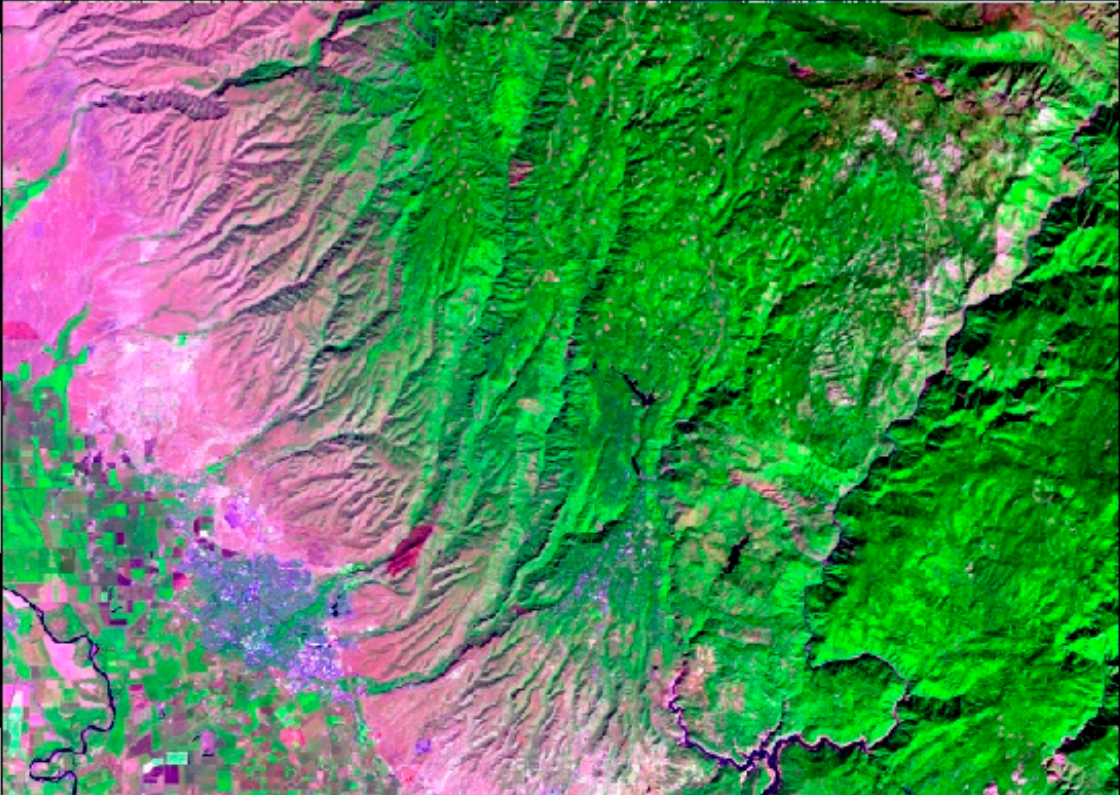
\includegraphics[width=0.49\textwidth]{resources/forest_map.png}\hfill
        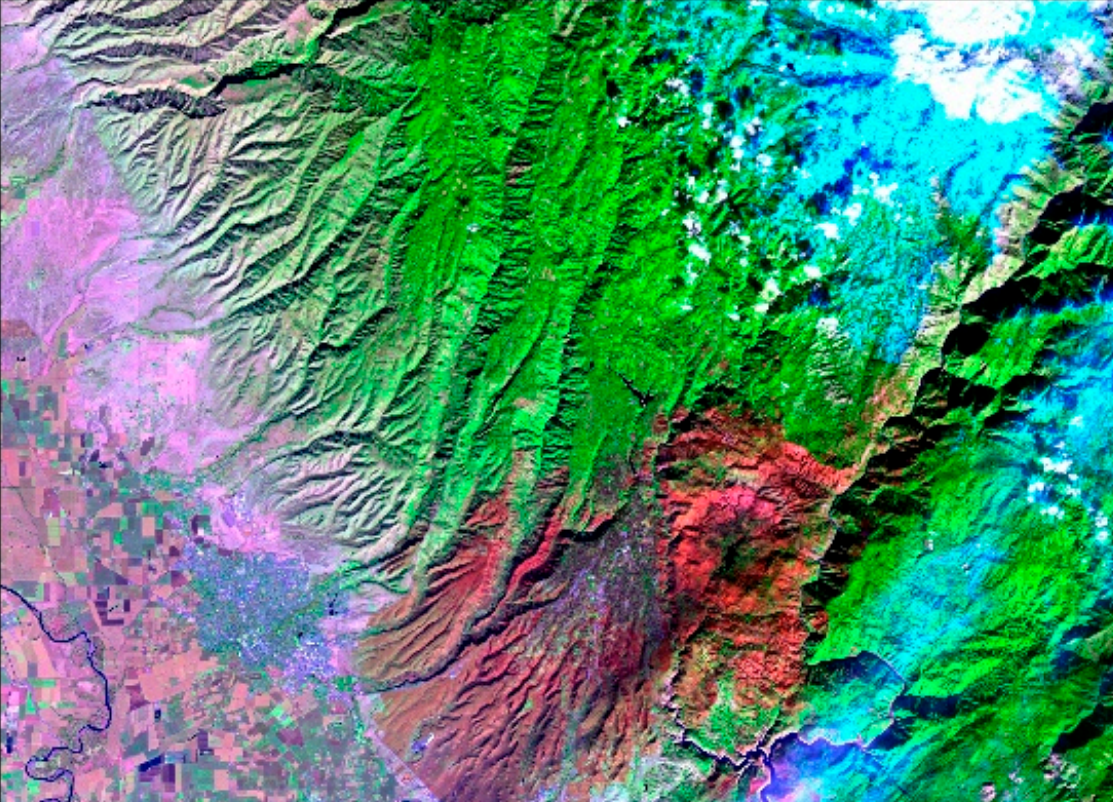
\includegraphics[width=0.49\textwidth]{resources/forest_map_burn.png}
        \caption{Zdjęcie satelitarne terenu w Buttle County (źródło: \cite{camp-fire-wildfire-in-california}), przed i po pożarze}
        \label{fig:buttle-county-fire-sat-photo}
    \end{figure}

\section{Zastosowane narzędzia oraz pozyskane dane}
\label{chap:tools-and-data}

    W celu przeprowadzenia symulacji rozprzestrzeniania się ognia skorzystaliśmy z solvera IGA-ADS \cite{iga-ads-solver-github}, który powstał do rozwiązywania niestacjonarnych problemów w \( L^2 \) stosując izogeometryczną metodę elementów skończonych (ang. \textit{isogeometric finite element method}) \cite{LOS201799}. Solver ten posiada zaprogramowaną funkcjonalność symulowania rozprzestrzeniania się ognia bazując na odpowiednio przygotowanej "mapie paliwa".
    
    Mapa jest wczytywana do kodu programu jako 2-wymiarowa tablica liczb zmiennoprzecinkowych znormalizowanych w zakresie \( [0,1] \) stworzona z obrazu terenu np. ze zdjęcia satelitarnego jak w przypadku naszego badania \ref{fig:buttle-county-fire-sat-photo}. Z założenia - im większa wartość danego pixela tym więcej jest w tym miejscu paliwa.

    Wyniki symulacji, które uzyskamy, możemy łatwo porównać z rzeczywistym przebiegiem pożaru ponieważ w artykule znajduje się także zdjęcie po pożarze, na którym widać wypalone obszary \ref{fig:buttle-county-fire-sat-photo}.
    
\section{Przygotowanie mapy dla solvera}
\label{sec:prepare-map-for-solver}
    Aby otrzymać taką mapę musieliśmy zdjęcie \ref{fig:buttle-county-fire-sat-photo} transformować do skali szarości a następnie stworzyć z niego plik tekstowy. Takie działanie uzyskaliśmy dzięki zastosowaniu prostego skryptu napisanego w języku Python.

\begin{lstlisting}[
    language=Python,
    caption={Skrypt do przetwarzania zdjęcia satelitarnego na dane dla solvera},
    label=lst:map-to-solver-data
]
import cv2
import matplotlib.pyplot as plt
import pandas as pd

im = cv2.imread("forest_map.png")
imbw = im[:, :, 1]  # only green channel
imbw = imbw.reshape(imbw.shape[0], imbw.shape[1])
imbw = imbw / 255
df = pd.DataFrame(imbw)
df.to_csv('image.csv', index=False, header=False)
\end{lstlisting}

    \begin{figure}[!htpb]
        \centering
        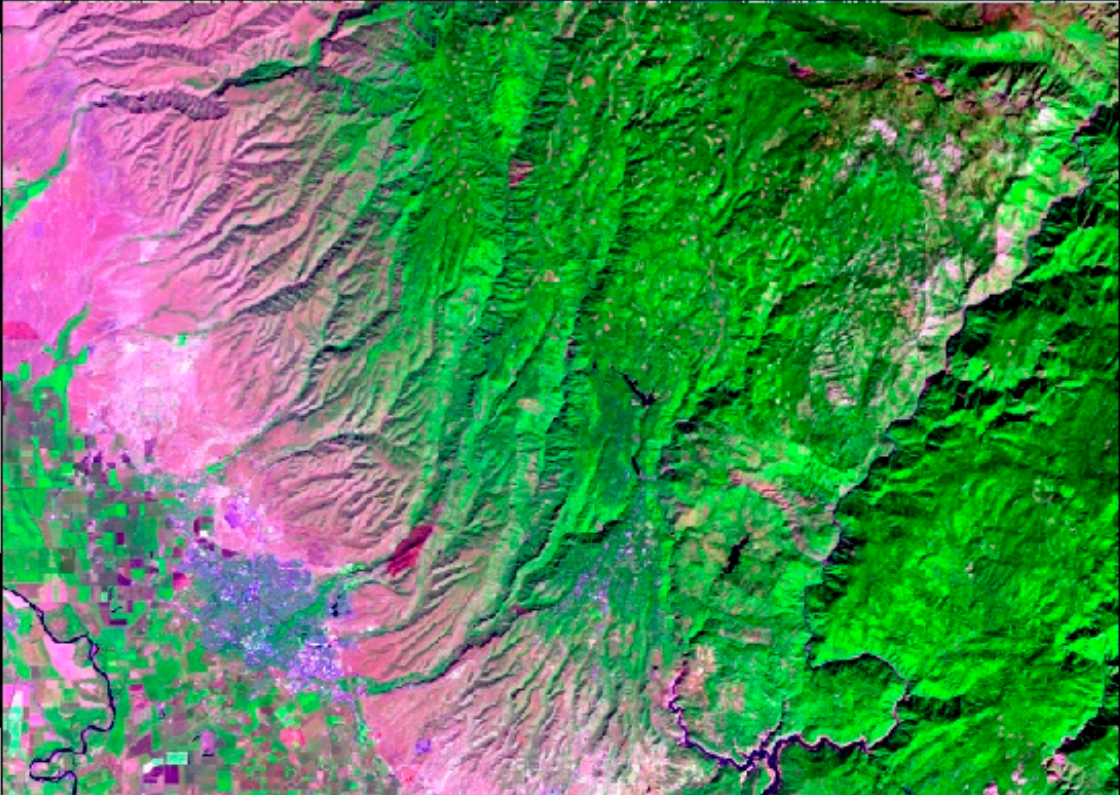
\includegraphics[width=0.49\textwidth]{resources/forest_map.png}\hfill
        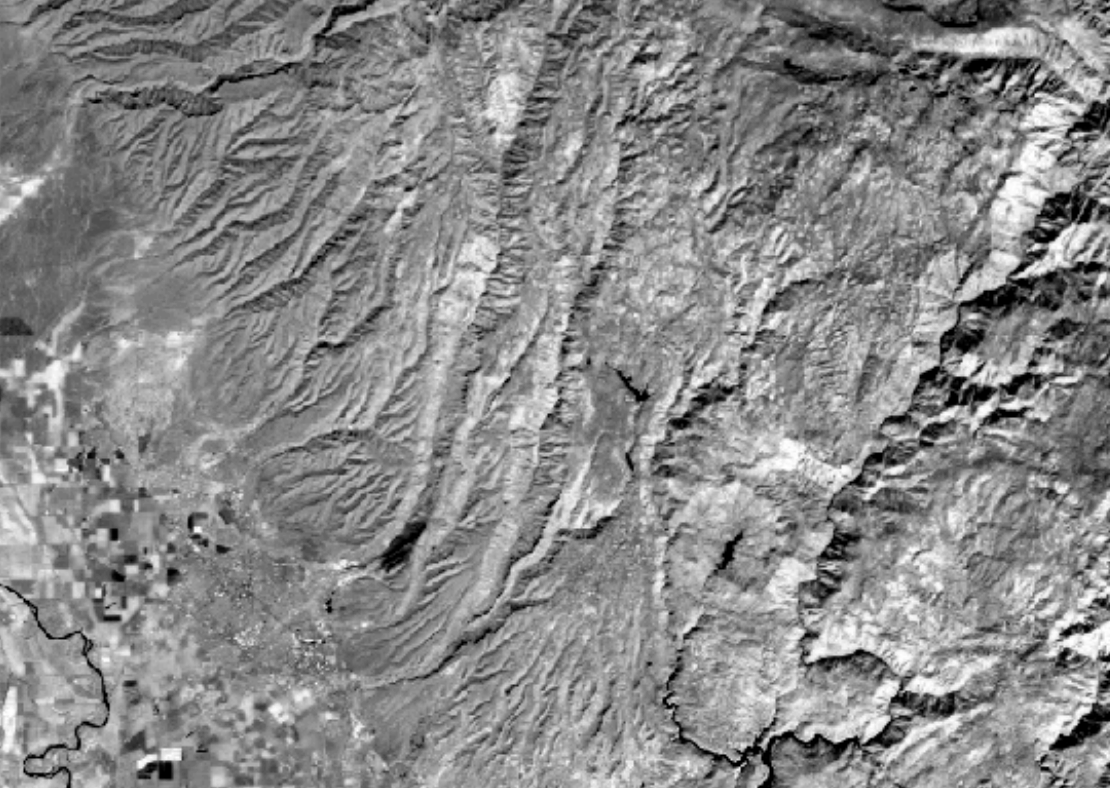
\includegraphics[width=0.49\textwidth]{resources/forest_map_gray.png}
        \caption{Porównanie zdjęcia satelitarnego wykonanego przed pożarem i mapy paliwa uzyskanej przez ekstrakcję koloru zielonego z tego zdjęcia.}
        \label{bw-comparison}
    \end{figure}

\section{Zmiany w kodzie symulacji}
Empirycznie wyznaczyliśmy następujące parametry programu, tak by wyniki symulacji były jak najbardziej zbliżone do zdjęcia satelitarnego po pożarze.
Zmieniliśmy wartość wektora wiatru \texttt{(bx, by)}, zmieniliśmy epicentrum i~rozmiar początkowego rozpaleniska i~dodaliśmy wczytywanie mapy terenu/paliwa z~wcześniej przetworzonego pliku \texttt{csv}.

\begin{lstlisting}[
    language=C,
    caption={Zmiany w kodzie symulacji},
    label=lst:code-changes
]
double bx = -6;
double by = -6;

double init_state(double x, double y) {
    x -= 17.0;
    y += 5.0;
    static constexpr auto r{5};
    static constexpr auto R{5};
    return T0 + Tcomb * bump(r, R, x, y);
};

void before() override {
    prepare_matrices();
    auto init = [this](double x, double y) { return init_state(x, y); };
    projection(u, init);
    solve(u);
    output.to_file(u, "out_0.data");

    const auto fuel_map{get_fuel_map()};

    const auto size_y{std::size(fuel_map)};
    const auto size_x{std::size(fuel_map[0])};

    const auto scale_x{static_cast<double>(size_x) / (x.b - x.a)};
    const auto scale_y{static_cast<double>(size_y) / (y.b - y.a)};

    auto fuel_init = [&](double x, double y) {
        const auto map_x{static_cast<std::size_t>(scale_x * x)};
        const auto map_y{static_cast<std::size_t>(scale_y * (Base::y.b - y))};

        if (map_x >= size_x || map_y >= size_y)
            throw std::runtime_error("Invalid map coordinates:...");

        return fuel_map[map_y][map_x] * 0.725;
    };
\end{lstlisting}

\section{Wyniki odpalenia symulacji}
\label{chap:results}

    Na rysunkach~\ref{frames-1}, \ref{frames-2}, \ref{frames-3} i~\ref{frames-4} prezentujemy kolejne klatki z~animacji symulacji pożaru lasu.
    Na rysunku porównujemy zdjęcie satelitarne wykonane po pożarze z~wynikami symulacji.

    \begin{figure}[!htpb]
        \centering
        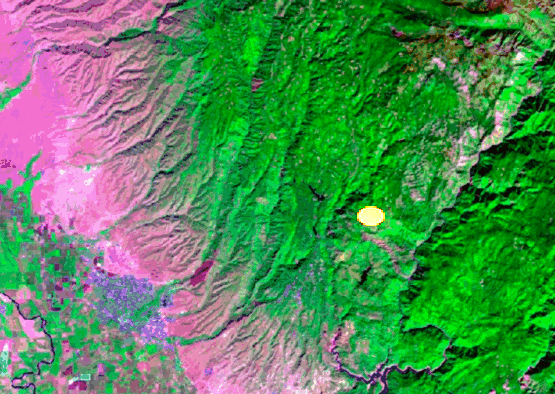
\includegraphics[width=0.49\textwidth]{resources/wildfire.overlay.000.png}\hfill
        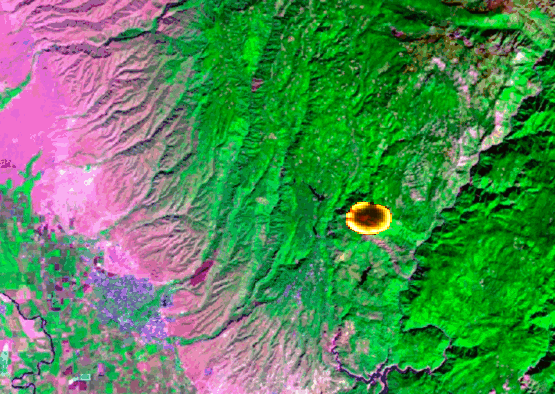
\includegraphics[width=0.49\textwidth]{resources/wildfire.overlay.007.png}
        \caption{Klatki z animacji symulacji pożaru lasu - cz. 1}
        \label{frames-1}
    \end{figure}

    \begin{figure}
        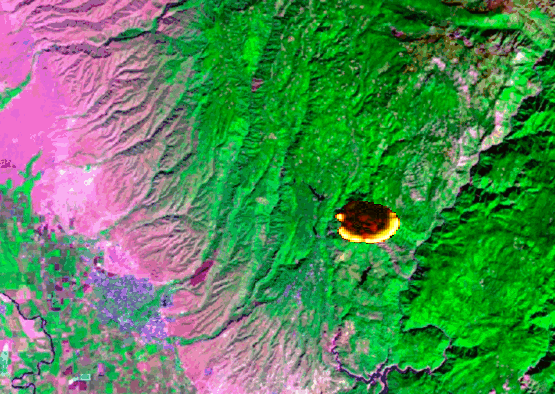
\includegraphics[width=0.49\textwidth]{resources/wildfire.overlay.015.png}\hfill
        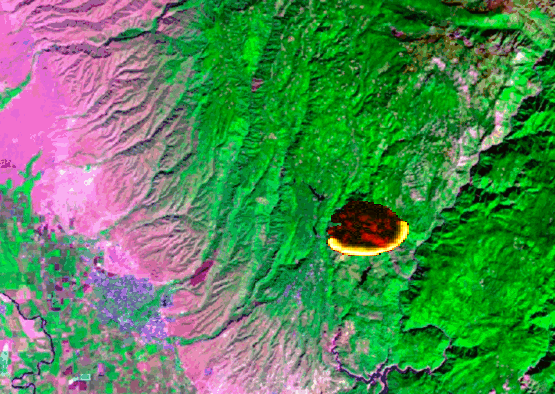
\includegraphics[width=0.49\textwidth]{resources/wildfire.overlay.026.png}        
        \\[\smallskipamount]
        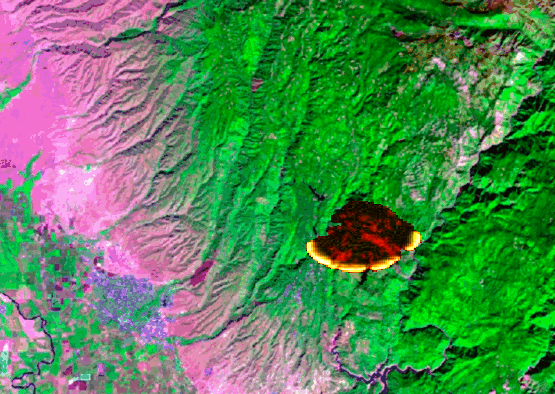
\includegraphics[width=0.49\textwidth]{resources/wildfire.overlay.040.png}\hfill
        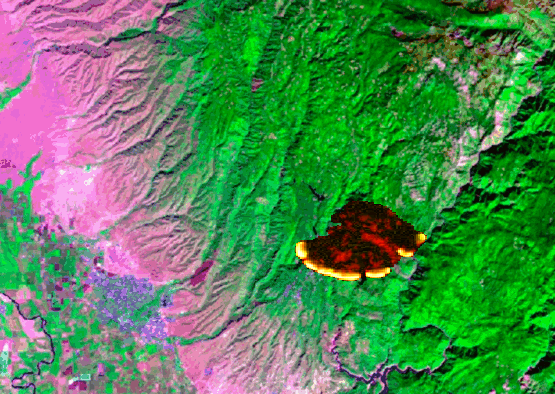
\includegraphics[width=0.49\textwidth]{resources/wildfire.overlay.047.png}
        \\[\smallskipamount]
        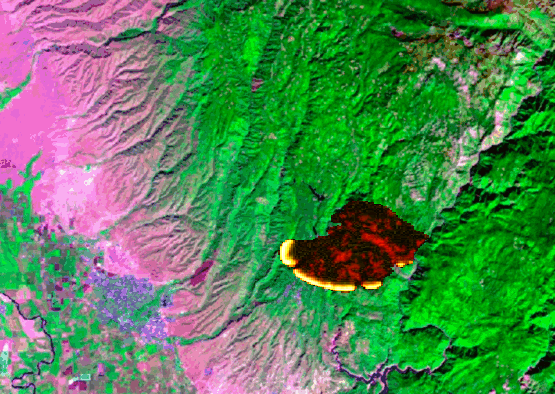
\includegraphics[width=0.49\textwidth]{resources/wildfire.overlay.057.png}\hfill
        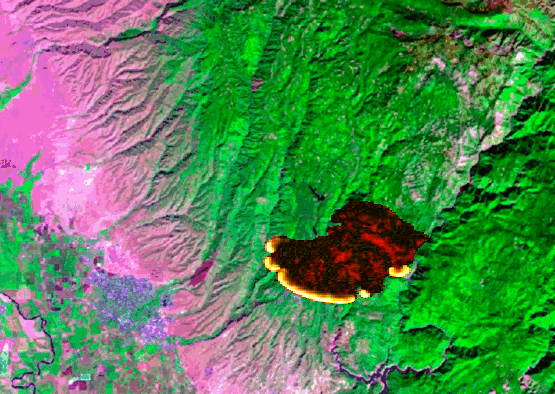
\includegraphics[width=0.49\textwidth]{resources/wildfire.overlay.068.png}
        \caption{Klatki z animacji symulacji pożaru lasu - cz. 2}
        \label{frames-2}
    \end{figure}

    \begin{figure}
        \centering
        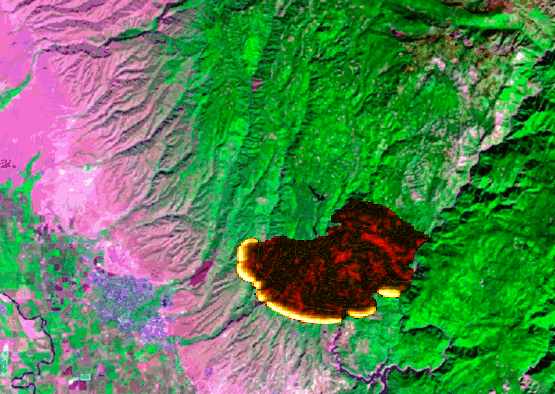
\includegraphics[width=0.49\textwidth]{resources/wildfire.overlay.086.png}
        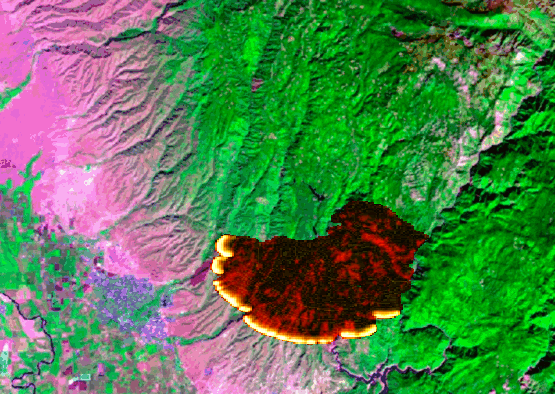
\includegraphics[width=0.49\textwidth]{resources/wildfire.overlay.104.png}\hfill
        \\[\smallskipamount]
        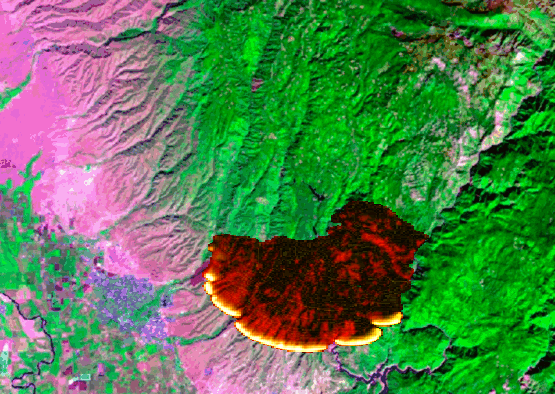
\includegraphics[width=0.49\textwidth]{resources/wildfire.overlay.111.png}\hfill
        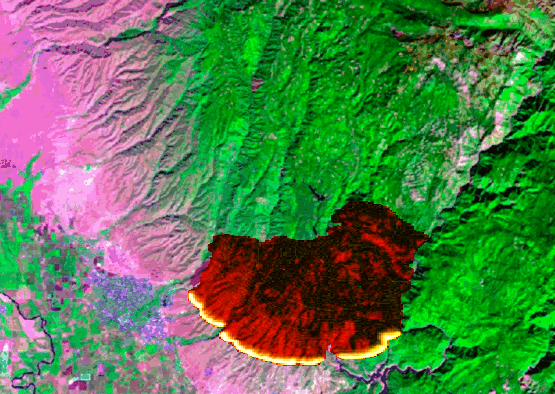
\includegraphics[width=0.49\textwidth]{resources/wildfire.overlay.123.png}
        \\[\smallskipamount]
        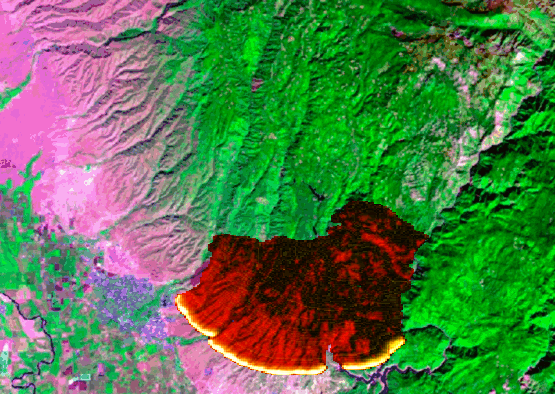
\includegraphics[width=0.49\textwidth]{resources/wildfire.overlay.132.png}\hfill
        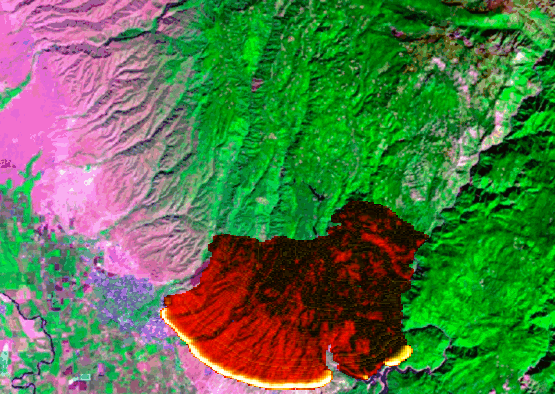
\includegraphics[width=0.49\textwidth]{resources/wildfire.overlay.144.png}
        \caption{Klatki z animacji symulacji pożaru lasu - cz. 3}
        \label{frames-3}
    \end{figure}

    \begin{figure}
        \centering
        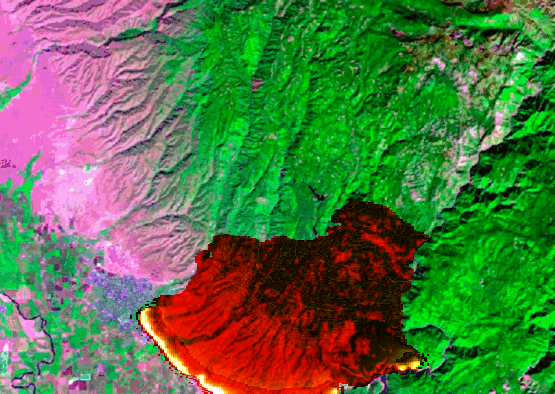
\includegraphics[width=0.49\textwidth]{resources/wildfire.overlay.158.png}
        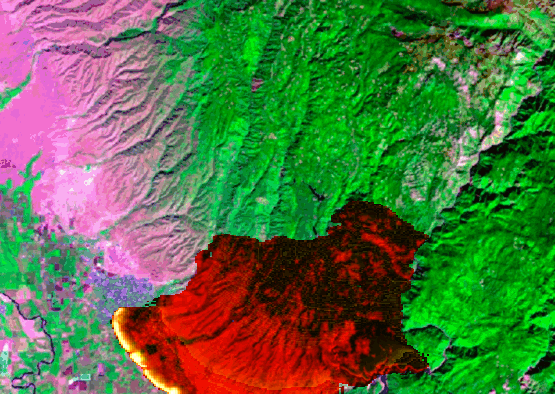
\includegraphics[width=0.49\textwidth]{resources/wildfire.overlay.176.png}\hfill
        \\[\smallskipamount]
        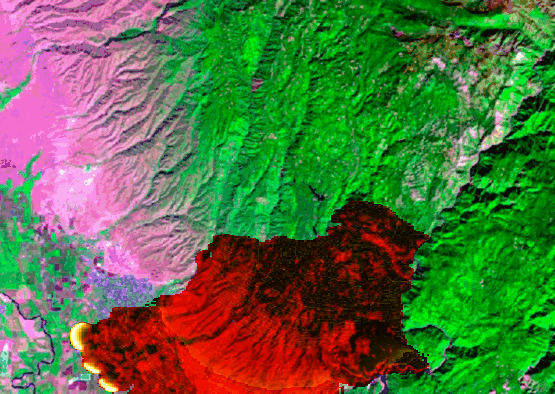
\includegraphics[width=0.49\textwidth]{resources/wildfire.overlay.203.png}\hfill
        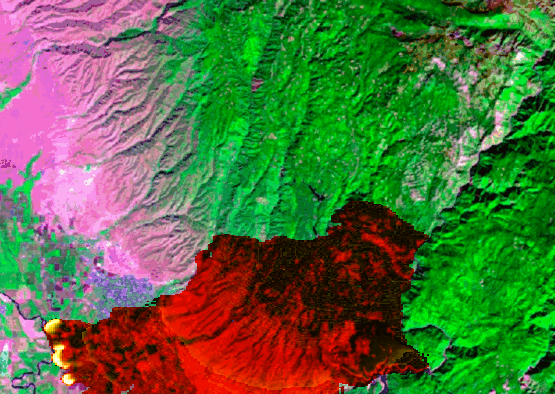
\includegraphics[width=0.49\textwidth]{resources/wildfire.overlay.221.png}
        \\[\smallskipamount]
        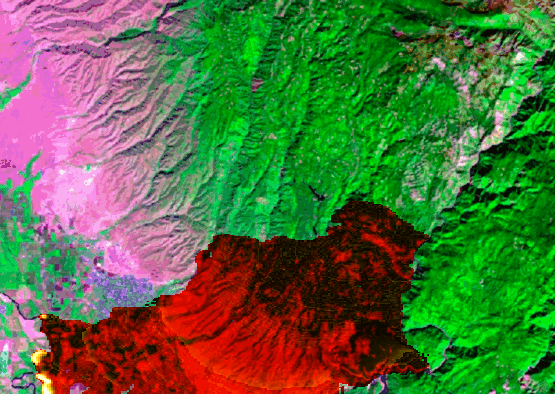
\includegraphics[width=0.49\textwidth]{resources/wildfire.overlay.236.png}\hfill
        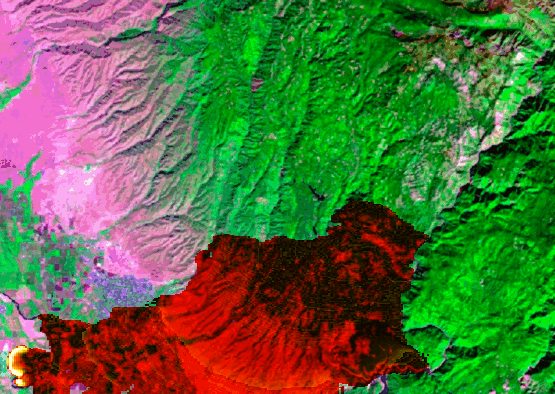
\includegraphics[width=0.49\textwidth]{resources/wildfire.overlay.251.png}
        \caption{Klatki z animacji symulacji pożaru lasu - cz. 4}
        \label{frames-4}
    \end{figure}

    \begin{figure}
        \centering
        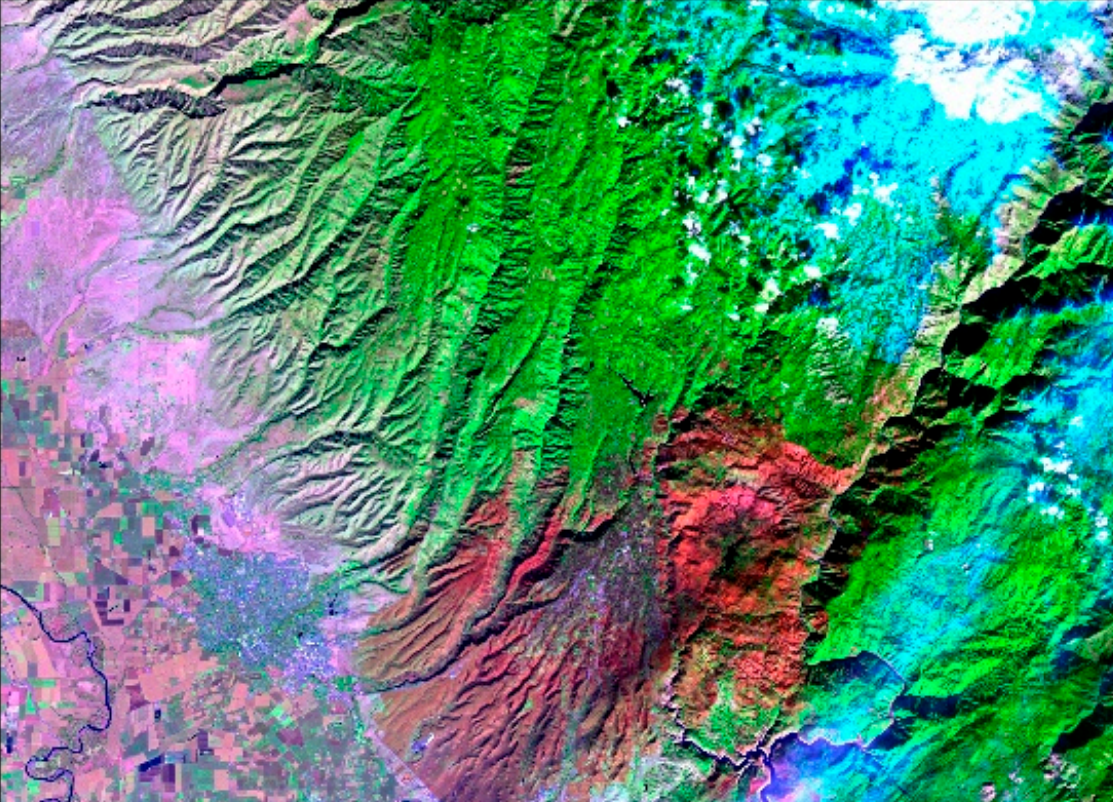
\includegraphics[width=0.49\textwidth]{resources/forest_map_burn.png}\hfill
        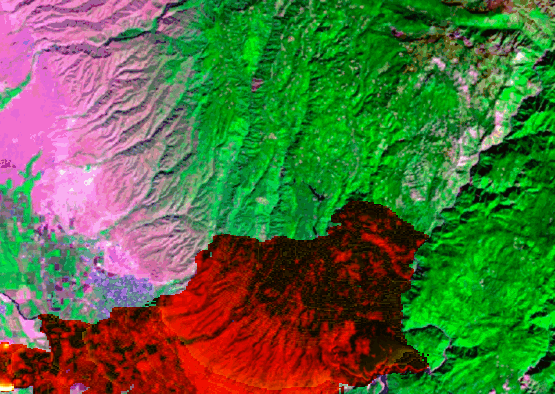
\includegraphics[width=0.49\textwidth]{resources/wildfire.overlay.266.png}
        \caption{Porównanie zdjęcia satelitarnego wykonanego po pożarze i wyników symulacji pożaru lasu.}
        \label{comparison}
    \end{figure}
% TO DO

\newpage
% \clearpage
 
\printbibliography

\end{document}
